\documentclass[a4paper,11pt]{scrartcl}

\usepackage[ngerman]{babel} 
\usepackage[T1]{fontenc}
\usepackage[utf8]{inputenc}
\usepackage{hyperref}

\usepackage{amsmath,amsfonts,amssymb}
\usepackage{graphicx}
\usepackage{siunitx}

\usepackage{epstopdf}

\setcounter{section}{8}


\begin{document}
\hfill Alexander Schnapp

\hfill Max Menges

\hfill introhpc02

\begin{center}
\underline{\Huge{Intro HPC: Blatt 8}}\\
\large{24.11.1014}\\
\end{center}


\subsection{Reading: GPU Computing}
In this article the author wants to give the reading a insight to the world of GPU computing. Thereby this paper is not focused on research but more on theaching.

After analysing the requirements to apply gpu computing and the hardware components of a gpu he explains
the essentials of programming on a GPU.
The main part of the paper is then about the applications of gpu computing. Examples out of the computational biophysics and other research areas are mentioned.


Furthermore he gives an short overview what gpu computing will look like in the future e.g. the trend of a higher bandwidth
path between CPU and GPU since the PCI Express bus
between CPU and GPU was and is still a bottleneck in many
applications today.

\subsection{Saxpy-CUDA implementation}
In this exercise a CUDA based implemation of the saxpy workload is diskussed. Varying the problem size on the x-axis from 1KB to 10 MB
we compare the CPU computing time with the GPU computing time on the y-axis. Both axes are in logarithmic scale. One can clearly see that the GPU computing time is neglegeble expescially at high problem sizes.

\begin{figure}[htbp]
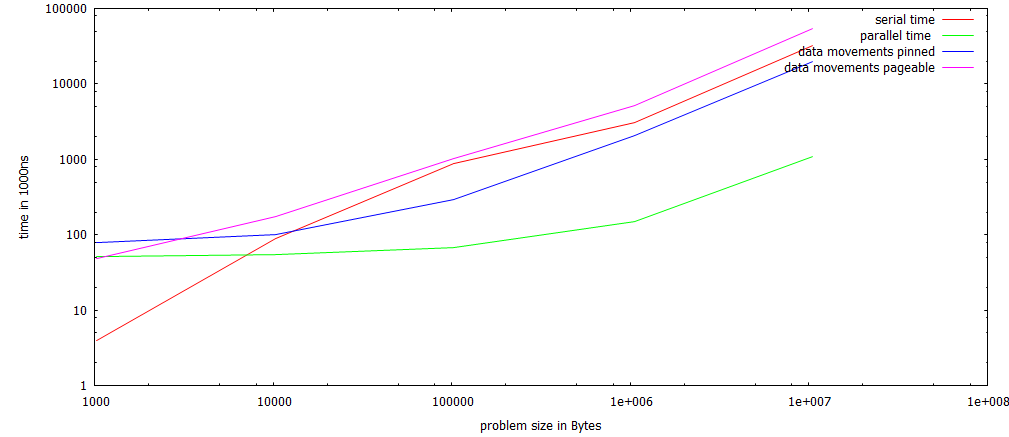
\includegraphics[width=\linewidth,
keepaspectratio]{vergleich}
\centering
\end{figure}

But you have to take care that for the GPU case you also have to consider the time of the datamovements from host to device and backwords. If you do so you see that the GPU is only in the case of a pinned memory and only except very small problem sizes faster than calculating on the CPU. 
\end{document}
